\section{False Discovery Rate}
\begin{frame}{Historia e Importancia}
	\begin{itemize}[<+- | alert@+>]
		
		\item La tasa de falsos descubrimiento (FDR) fue propuesto por primera vez por Benjamini and Hochberg (1995), la cual se colocó como una de las piezas clave en la investigación relacionada con FDR.
		
		\item Hasta antes de dicha publicación, la mayor parte de la inferencia relacionada con PHM se hacía fundamentalmente con base en métodos relacionados con el control de FWER, o bien técnicas similares derivadas de modificaciones a la misma. 
		
	\end{itemize}

\end{frame}

\begin{frame}
	\begin{df}
		Si definimos la variable aleatoria $Q$ como:
            \begin{align} \label{e_fdr}
                Q=\left\{ \begin{array}{cc}
                V/R & R>0\\
                0 & R=0
            \end{array} \right.
            \end{align}
        Entonces, se tiene que 
            \begin{align*}
                FDR = \mE(Q)=\mE\left( \frac{V}{V+S}\right)=\mE\left( \frac{V}{R} \right).
            \end{align*}
	\end{df}
	        Por como esta definido $Q$ (\ref{e_fdr}), tenemos que 
            \begin{align}\label{igudaldad_Q}
                \nonumber FDR=\mE\left( \frac{V}{R} \right) &= \mE\left( \frac{V}{R}\left| R>0\right. \right)\mP(R>0)+\mE\left( \frac{V}{R}\left| R=0\right. \right)\mP(R=0)\\
                &= \mE\left( \frac{V}{R}\left| R>0\right. \right)\mP(R>0).
            \end{align}
\end{frame}

\begin{frame}{Relación de FDR y FWER.}
	\begin{enumerate}[<+- | alert@+>]
		
		\item Si todas las hipótesis nulas son verdaderas, entonces controlar la FDR es equivalente a controlar la FWER.
		\item[] \textbf{Demostración.} Si todas las hipótesis nulas son verdaderas entonces $V=R$. Si $V=0$ entonces $\frac{V}{R}=0$ y si $V>0$ entonces $\frac{V}{R}=1$, por lo que (utilizando el resultado de (\ref{igudaldad_Q}))
            \begin{align*}
            FDR &= \mE\left( \frac{V}{R}\left| V=0\right. \right)\mP(V=0)+\mE\left( \frac{V}{R}\left| V>0\right. \right)\mP(V>0)\\
            &=0\times \mP(V=0)+1\times \mP(V\geq 1)\\
            &= \mP(V\geq 1)\\
            &= FWER.\ \ \finf
            \end{align*}

	\end{enumerate}
\end{frame}

\begin{frame}
	\begin{enumerate}[<+- | alert@+>]
		\item[2.] Si controlamos el FWER (es decir, lo mantenemos por debajo de algún valor $q^*$), entonces estamos controlando también FDR.
		\item[] \textbf{Demostración.} Si no todas las hipótesis nulas son verdaderas, entonces $V<R$ y  $\frac{V}{R}<1$, y esto implica que $\mE\left( \frac{V}{R} |V\geq 1\right)<1$. Ocupando lo anterior tenemos
            \begin{align*}
                FDR&= \mE\left( \frac{V}{R}\left| V=0\right. \right)\mP(V=0)+\mE\left( \frac{V}{R}\left| V\geq 1\right. \right)\mP(V\geq 1)\\
                &=0\times \mP(V=0)+\mE\left( \frac{V}{R}\left| V\geq 1\right. \right)\mP(V\geq 1)\\
                &<FWER.\ \ \finf
            \end{align*}
	\end{enumerate}
\end{frame}

\begin{frame}
	\begin{itemize}[<+- | alert@+>]
		
		\item Decimos por tanto que los procedimientos para el control FWER resultan ser más conservativos, en el sentido de que rechazan en promedio un menor número de hipótesis, que los procedimientos que controlan a FDR. 
		
	\end{itemize}

\end{frame}


\begin{frame}{Procemiento de control FDR de Benjamini y Hochberg(BH)}
    Considere la pruebas $H_1, H_2, ..., H_m$, basado en los p$-$values correspondientes $P_{1}, P_{2},..., P_{m}$. Entonces primero ordenemos los p$-$values, es decir, $P_{(1)}\leq P_{(2)}\leq \cdots \leq  P_{(m)}$ denotar por la hipótesis nula $H_{(i)}$ correspondiente a $P_{(i)}$. Defina el siguiente procedimiento de prueba múltiple de B$-$H:\\
\begin{align}
 \nonumber\text{sea k la $i$ más grande para la cual }P_{(i)}\leq \frac{i}{m}q*;\\
 \text{luego rechaza todo }H_{(i)} = 1, 2, ..., k.
\end{align} 
\end{frame}

\begin{frame}
    \begin{thh} \label{t_1}
Para estadísticos de prueba independientes y para cualquier configuración de hipótesis nulas falsas, el procedimiento anterior controla el FDR en $q*$.
    \end{thh}
\textbf{Demostración.} El teorema se deriva del siguiente lema.
\end{frame}

\begin{frame}
    \begin{lm} \label{l_1}
Para cualquier $0 <m_0 <m$ p-values independientes correspondientes a hipótesis nulas verdaderas, y para cualquier valor que puedan tomar los p-values de $m_1= m - m_0$ correspondientes a las hipótesis nulas falsas, el procedimiento de prueba múltiple definido por el procedimiento$(1)$ anterior satisface la desigualdad
\begin{equation}\label{2}
\mE (Q | P_{m_0+1}=p_1, ..., P_m = p_{m_1})\leq \frac{m_0}{m} q^*
\end{equation}
Ahora, suponga que $m_1=m-m_0$ algunas de las hipótesis son falsas. Cualquiera que sea la distribución conjunta de $P_1'' ,\cdots, P_{m_1}''$, que corresponde a estas falsas hipótesis, integrando la desigualdad (\ref{2}) anterior obtenemos
\begin{equation*}
\mE(Q) <\frac{m_0}{m}q* <q *,
\end{equation*}
y el FDR está controlado.
    \end{lm}
\end{frame}
\begin{frame}{Ejemplo para controlar la FDR con el procedimiento B-H}
    Neuhaus (1992 ) quiere probar los efectos de una nueva administración de carga frontal de $rt-PA$ vs el efecto clasico de administrar APSAC en la reducción de la mortalidad en el infarto miocardio.  \\
    
    El control de FDR es deseable ya que no se quiere concluir que el nuevo tratamiento sea mejor si es simplemente equivalente al tratamiento anterior en todos los aspectos (eventos cardíacos)
\end{frame}

\begin{frame}{Transiciones}
	\begin{itemize}[<+- | alert@+>]
		
		\item Los p$-$values individuales que reportan para cada prueba de hipótesis son 
		\item[] \begin{align*}
0.0001, 0.0004, 0.0019, 0.0095, 0.0201, 0.0278, 0.0298,\\ 0.0344, 0.0459, 0.3240, 0.4262, 0.5719, 0.6528, 0.7590, 1.000.
\end{align*}

\item Y los autores concluyen que:

\item[] ''\textit{En comparación con el tratamiento con APSAC, a pesar de más reoclusiones tempranas, el curso clínico con el tratamiento con rt-PA es más favorable con menos complicaciones hemorrágicas y una tasa de mortalidad hospitalaria sustancialmente más baja, presumiblemente debido a una mejor permeabilidad temprana de la arteria relacionada con el infarto}''.
	\end{itemize}

\end{frame}

\begin{frame}
    \begin{rr}
    En el estudio no se especifíca cual fue el estadístico de prueba que utilizaron.
    \end{rr}
    Realizemos las metodología de Bonferroni y $B-H$ para controlar las diferentes tasas. Es decir, para controlar la FWER considerando $\alpha=0.05$ rechazamos si
    
    $$p_i<0.05/15=0.0033.$$
    Y para controlar la FDR con $q^*=0.05$ y sea $k$ la $i$ más grande para el cual $p_{(i)}\leq \frac{i}{m}q^*$, entonces rechzamos todas las $H_{(i)}=1,2,\cdots, k.$

\end{frame}

\begin{frame}
\begin{table} \label{t_p_ejecicio}
\begin{tabular}{ccccccccc}
\hline
\hline
$H_{0i}$ & p$-$values  &  Umb. BH & Umb. Bonferr. & R BH& R Bonferr.\\
\hline
\hline
1 &   0.0001& 0.0034&       0.0033&       TRUE&               TRUE\\
2 &   0.0004& 0.0067&       0.0033&       TRUE&               TRUE\\
3 &   0.0019& 0.0100&       0.0033&       TRUE&               TRUE\\
4 &   0.0095& 0.0134&       0.0033&       TRUE&              FALSE\\
5 &   0.0201& 0.0167&       0.0033&      FALSE&              FALSE\\
6 &   0.0278& 0.0200&       0.0033&      FALSE&              FALSE\\
7 &   0.0298& 0.0234&       0.0033&      FALSE&              FALSE\\
14&   0.7590& 0.0467&       0.0033&      FALSE&              FALSE\\
15&   1.0000& 0.0500&       0.0033&      FALSE&              FALSE\\
\hline
\hline
\end{tabular}
\caption{Resultados de los p$-$values.}
\end{table}
\end{frame}

\begin{frame}

	\begin{itemize}[<+- | alert@+>]
		\item Las primeras tres hipótesis corresponden a una reacción alérgica reducida y a dos aspectos diferentes del sangrado; no incluyen la comparación de mortalidad. Por tanto, la afirmación sobre una reducción significativa de la mortalidad no está justificada desde el punto de vista clásico. Pero controlando el FDR rechazamos la hipótesis 4.
		\item En la figura (\ref{comparacion_metodos}) observamos los "umbrales" para rechazar la hipótesis nula  para las distintas metodologías. Se observa claramente que las metodologías para controlar el $FWER$ resultan más conservadoras ya que tiene un umbral muy pequeño para rechazo, en cambio si se controla el $FDR$ el umbral es 0.5.
	\end{itemize}

\end{frame}

\begin{frame}
\begin{figure}[H]
\centering \label{comparacion_metodos}
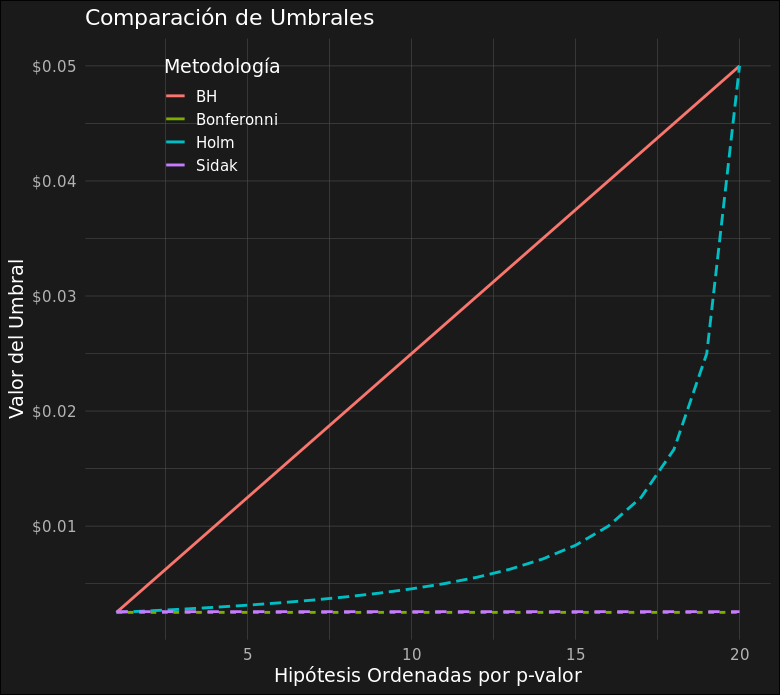
\includegraphics[scale=.39]{comparacion_de_metodos.png}
\caption{Comparación del valor del Umbral de rechazo}
\end{figure}
\end{frame}

\section{MCP - Ciencia de datos.}
\begin{frame}{Aplicación del control FDR en neurociencia}
    
    	\begin{itemize}[<+- | alert@+>]
		
		\item En este ejemplo, se realizó un análisis de las masas en imágenes de resonancia magnética (RM) extraídas de la iniciativa de datos abiertos de la serie de acceso abierto de estudios de imágenes (OASIS). Estos datos contienen imágenes ponderadas en T1 de 416 participantes con y sin demencia de entre 18 y 96 años, lo que permite investigar cómo la edad y las enfermedades relacionadas \textbf{con la edad influyen en la morfología cerebral}.\\
		\item El objetivo del estudio fue determinar que partes del cerebro están relacionadas de su edad.
	\end{itemize}

\end{frame}

\begin{frame}{Metodología}
    
    \begin{itemize}[<+- | alert@+>]
		
		\item Para descargar el conjunto de datos de OASIS, visite $http://www.oasis-brains.org/\#data$ y elija el lanzamiento OASIS-1, que contiene imágenes de resonancia magnética (MR) de 416 participantes de entre 18 y 96 años. El archivo de información del participante incluye variables demográficas básicas (edad, género, mano de obra, nivel educativo, estatus socioeconómico), variables clínicas y estimaciones de volumen cerebral. 
		
		\item[] \begin{figure}[H]
\centering 
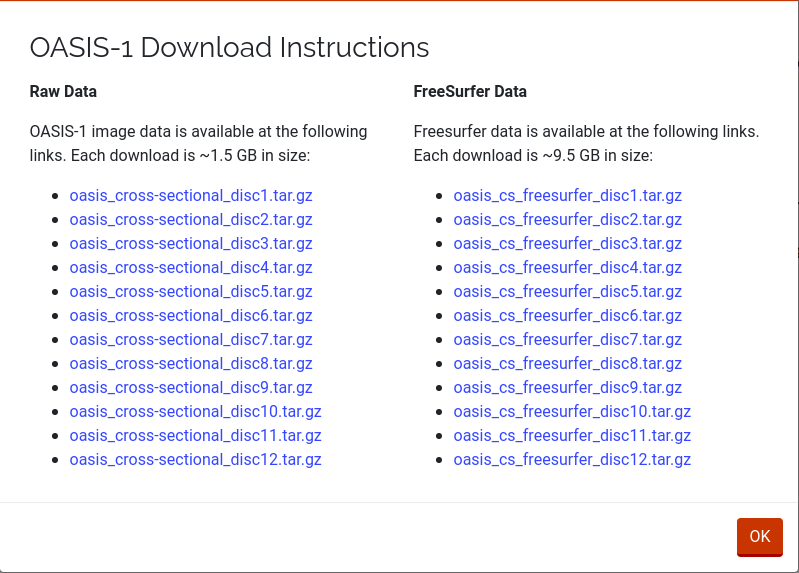
\includegraphics[scale=.19]{descarga_datos.png}
\end{figure}
	\end{itemize}
\end{frame}

\begin{frame}
    Se considero calcular los coeficientes de correlación Spearman  entre el grosor cortical y la edad en cada vóxel cortical, y se consideraron 163810 pruebas de la siguiente forma
\begin{align*}
H_{0i}: \rho_s =0 \ \ \ vs \ \ \ H_{0i}:\rho_s\neq 0, \ \ \forall i=1,\cdots, 163810.
\end{align*}
donde $\rho_s=1-\frac{6\sum d_i^2}{n(n^2-1)}$ y $d_i=rg(X_i)-rg(Y_i)$ es la diferencia de los rangos de cada observación. Se puede probar que si $n$ es grande entonces 
$$\rho_s\sqrt{\frac{n-2}{1-\rho_s^2}} \sim t_{n-2}$$
\end{frame}

\begin{frame}
    \begin{itemize}[<+- | alert@+>]
		
		\item Considerando lo anterior procedió a calcular los p$-$values de cada juego de hipótesis. Y posterior se le aplicaron las correcciones de Sidák para controlar el family$-$wise error rate (FWER), y el procedimiento BH para controlar la FDR. 
		
		\item Un total del $55\%$ de los vóxel mostró un efecto estadísticamente significativo del envejecimiento sobre el grosor cortical usando la corrección de Sidak. Por el contrario, cuando la corrección se basó en el procedimiento Benjamini-Hochberg, el número de vértices significativos fue del $82\%$, lo que sugiere un efecto más generalizado. El nivel crítico sin corregir se fijó en $\alpha = 0.05$ en ambos análisis.
	\end{itemize}
    
\end{frame}

\begin{frame}{Comparación}
Los resultados se muestran en la figura (\ref{cerebro}), lo cuál podemos concluir que algunos de los mayores efectos relacionados con la edad se observan en el surco central.
    \begin{figure}[H]
        \centering \label{cerebro}
        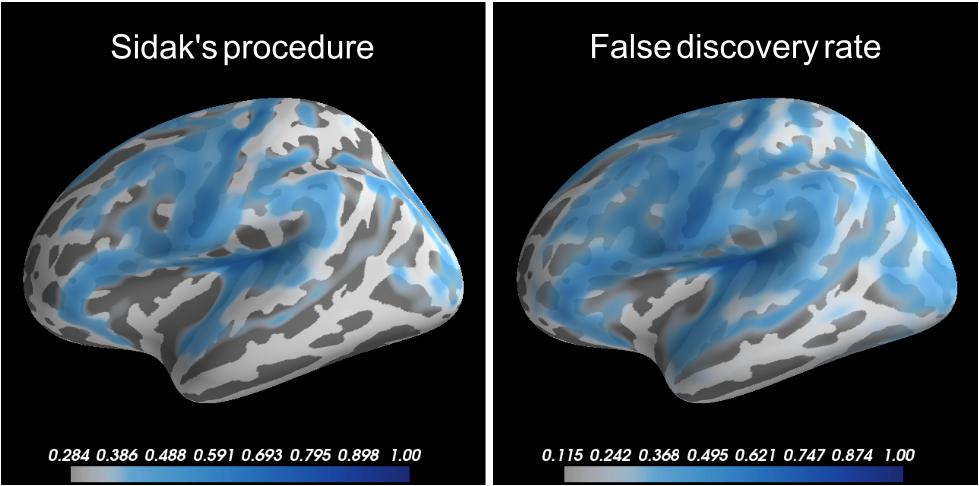
\includegraphics[scale=.29]{neurociencia_FDR_FWER.png}
        \caption{Diferencias cuando se controla el FWER y el FDR.}
    \end{figure}
\end{frame}

\begin{frame}{Artículos interesantes de ejemplos...}
    \begin{itemize}[<+- | alert@+>]
	\item Y. Benjamini and Y. Gavrilov, A Simple Forward Selection Procedure Based On False Discovery Rate Control(2009). 
	
	\item Christopher J. Miller (1) et. al., Controling the False-Discovery Rate in Astrophysical Data Analysis(2001). 
	
	'\textit{El propósito de este artículo es presentar el procedimiento FDR a la comunidad astrofísica. Ilustramos el poder de FDR a través de varios ejemplos astronómicos, incluida la detección de características frente a una función unidimensional suave, por ejemplo, ver las \textit{ondulaciones de bariones} en un espectro de potencia de fluctuaciones de materia y detección de píxeles de origen en datos de imágenes...}'
	\end{itemize}
\end{frame}


\begin{frame}{Conclusiones}
    
    \begin{itemize}[<+- | alert@+>]
	\item Se presentaron las bases teóricas sobre las pruebas de hipótesis múltiples desde el enfoque clásico controlando la $FWER$ y la revolucionaria idea que propusieron Benjamini y Hochberh [1995] sobre controlar la $FDR$.
	
	\item La teórica presentada en este documento como se mencionó son las bases de $MCP$, en la actualidad ya existen una gran variedad de metodologías para controlar $FDR$ y $FWER$ la mayoría es son modificaciones del método de Bonferroní y $BH$.
	\end{itemize}
	
\end{frame}